\documentclass[12pt, a4paper]{article}
 
\usepackage[top=1in, bottom=0.9in, left=0.95in, right=0.95in]{geometry} 
\usepackage{amsmath,amsthm,amssymb,mathtools}
\usepackage{listings}
%\usepackage[ngerman]{babel}
\usepackage{graphicx}
\usepackage{subcaption}
\usepackage{harpoon}

\newcommand{\vect}[1]{\overrightharp{\ensuremath{#1}}}
\newcommand{\field}[1]{\par\begin{large}{\vspace*{0.5cm}\noindent{}\textbf{#1}\vspace*{-1mm}}\end{large}}
\newcommand{\rom}[1]{\uppercase\expandafter{\romannumeral #1\relax}}
%\newcommand{\problem}[2]{{\par\noindent{}\textit{Problem {\uppercase\expandafter{\romannumeral #1\relax}}.} #2}}
\newenvironment{problem}[3]{{\par\vspace*{4.5mm}\noindent{}\textit{Problem {\uppercase\expandafter{\romannumeral #1\relax}}:} #2}\vspace*{-0.2cm}\hfill{\textit{{#3} Points.}}\\\hspace*{0.8cm}\hfill\begin{minipage}{\dimexpr\textwidth-1.3cm}}{\end{minipage}\hspace*{0.5cm}}
% don't fucking ask! (im 4h into this and it __works__)
 
\lstset{literate=
  {ä}{{\"a}}1 {ö}{{\"o}}1 {ü}{{\"u}}1
  {Ä}{{\"A}}1 {Ö}{{\"O}}1 {Ü}{{\"U}}1
  {ß}{{\ss}}1
}

\begin{document}

\title{Delightful Mathematical Problems}
\author{Philip Gei\ss{}ler}
 
\maketitle

\field{Real Analysis}
\begin{problem}{1}{Commutative Exponentiation}{3}
\begin{align*}
p^q &= q^p & p,q\in\mathbb{R}^+
\end{align*}
Find the functions $p(q)$ or $p(c), q(c)$ which satisfy the given equation. Where do they intersect? Give the Point $(p,q)$.
\end{problem}

\begin{problem}{2}{Implicit Function}{4}
\begin{align*}
\varphi_\mathbb{Q} :&\mathbb{~~Q} \longmapsto \mathbb{Q} &\varphi_\mathbb{Q}(p)\cdot\varphi_\mathbb{Q}(q) &= \varphi_\mathbb{Q}(p+q)\\
\varphi_\mathbb{R} :&\mathbb{~~R} \longmapsto \mathbb{R} &\varphi_\mathbb{R}(p)\cdot\varphi_\mathbb{R}(q) &= \varphi_\mathbb{R}(p+q)
\end{align*}
Which function do both functions $\varphi(x)$ represent? Are they continuous? 
\end{problem}


\field{Number Theory}
\begin{problem}{3}{A Stack of Sums}{5}
\begin{align*}
\mathcal{S}_{n}^\infty \coloneqq {\text{\hspace{-4.9mm}}\sum\limits^{\infty}_{\phantom{...}\begin{smallmatrix*}x_i\!&=&\!x_{i-1}\\x_1\!&=&\!0\hfill\end{smallmatrix*}}}^{\text{\hspace{-5mm}}\sum\limits^{n}_{i=1}}\hspace{1mm}\frac{1}{2^{x_i}} \coloneqq \sum^{\infty}_{x_1 = 0}\sum^{\infty}_{x_2 = x_1}\cdots\hspace{-2.3mm}\sum^{\infty}_{x_n = x_{n-1}}\frac{1}{2^{x_n}}
\end{align*}
What are the values of $\mathcal{S}_{1}^\infty$, $\mathcal{S}_{2}^\infty$ and $\mathcal{S}_{3}^\infty$? Does $\mathcal{S}_{n}^\infty$ converge for all $n\in\mathbb{N}$? If so, can you give a general answer for $\mathcal{S}_{n}^\infty$?
\end{problem}

\begin{problem}{4}{Mo Money Mo Bills}{3}
\begin{align*}
\mathcal{P}_{n_0} &= \left\lbrace{\mathcal{S}\mid \mathcal{S}\subseteq \mathbb{N},~ \forall n\in\mathbb{N},~ n<n_0,~ \exists s_1,s_2.\dots,s_x \in \mathcal{S}: \textstyle\sum_{i=1}^xs_i=n}\right\rbrace
\end{align*}\vspace*{-0.9cm}\begin{align*}
\overline{\mathcal{P}}_{n_0} &= \min\{|\mathcal{S}| \mid \mathcal{S}\in\mathcal{P}_{n_0}\} &\mathcal{R}_x &= \lim_{{n_0}\rightarrow \infty} \frac{\overline{\mathcal{P}}_{n_0}}{n_0}
\end{align*}
You have a purse that can fit $x$ bills, but you want to be able to pay every possible integer amount of money in one go. Fortunately you are able to print every bill of integer value you want. What is the smallest ratio $\mathcal{R}_x$ for $x\in\mathbb{N}$ of new bills per possible payable amount of money you need to print if your spendings can be arbitrarily large?
\end{problem} 
\\ % for new Page

\field{Geometry}
\begin{problem}{5}{Infinite Curling}{2}
\vspace*{0.3cm}
You are playing Curling on an infinite sheet of ice with a circular Curling stone. To minimize the friction you are allowed to place infinite infinitesimally small frozen driblets $\mathcal{D}$ in some arragement on the ice, leading to a smaller contact area of just $\mathcal{X}$ times the area of the driblets. What is the smallest average number $\overline{\mathcal{X}}$ of driblets contacting the Curling stone you can reach if the stone's resting position must be stable on every point of the plane?

Stability means that for every point $P\in\mathbb{R}^2$ on the plane some driblets $\mathcal{D}_P = \{ d \mid d\in \mathcal{D}, (P_x-d_x)^2+(P_y-d_y)^2\leqslant 1\}$ will be supporting the Curling stone so that the center of gravity rests on the shape traced by the covered driblets (the smallest convex polygon $p\subset\mathbb{R}^2$ containing every driblet in $\mathcal{D}_P$) so that the Stone rests on top of them without tiping.
\end{problem}   

\begin{problem}{6}{Sierpinski's Rotational Inertia}{3}
\begin{align*}
\Theta &= \iiint_V\vect{r}_{\perp}^2\varrho(\vect{r}) dV = \varrho\iiint_V r^2 dV = \frac{m}{A\text{\,d}f}{\text{\,d}f}\iint_A r^2 dA = \frac{m}{A}\iint_A r^2 dA\\ \Theta_p &= \Theta_c + md_{p,c}^2 \text{~~~for parallel axes through $p$ and the center of gravity $c$}
\end{align*}
Calculate the moment of inertia of a Sierpinski triangle with mass $m$ and side length $l$ rotating about a rotational axis through its center of gravity and perpendicular to its plane.
\end{problem}

\begin{figure}
\vspace*{1cm}
\begin{subfigure}{.5\textwidth}
\centering
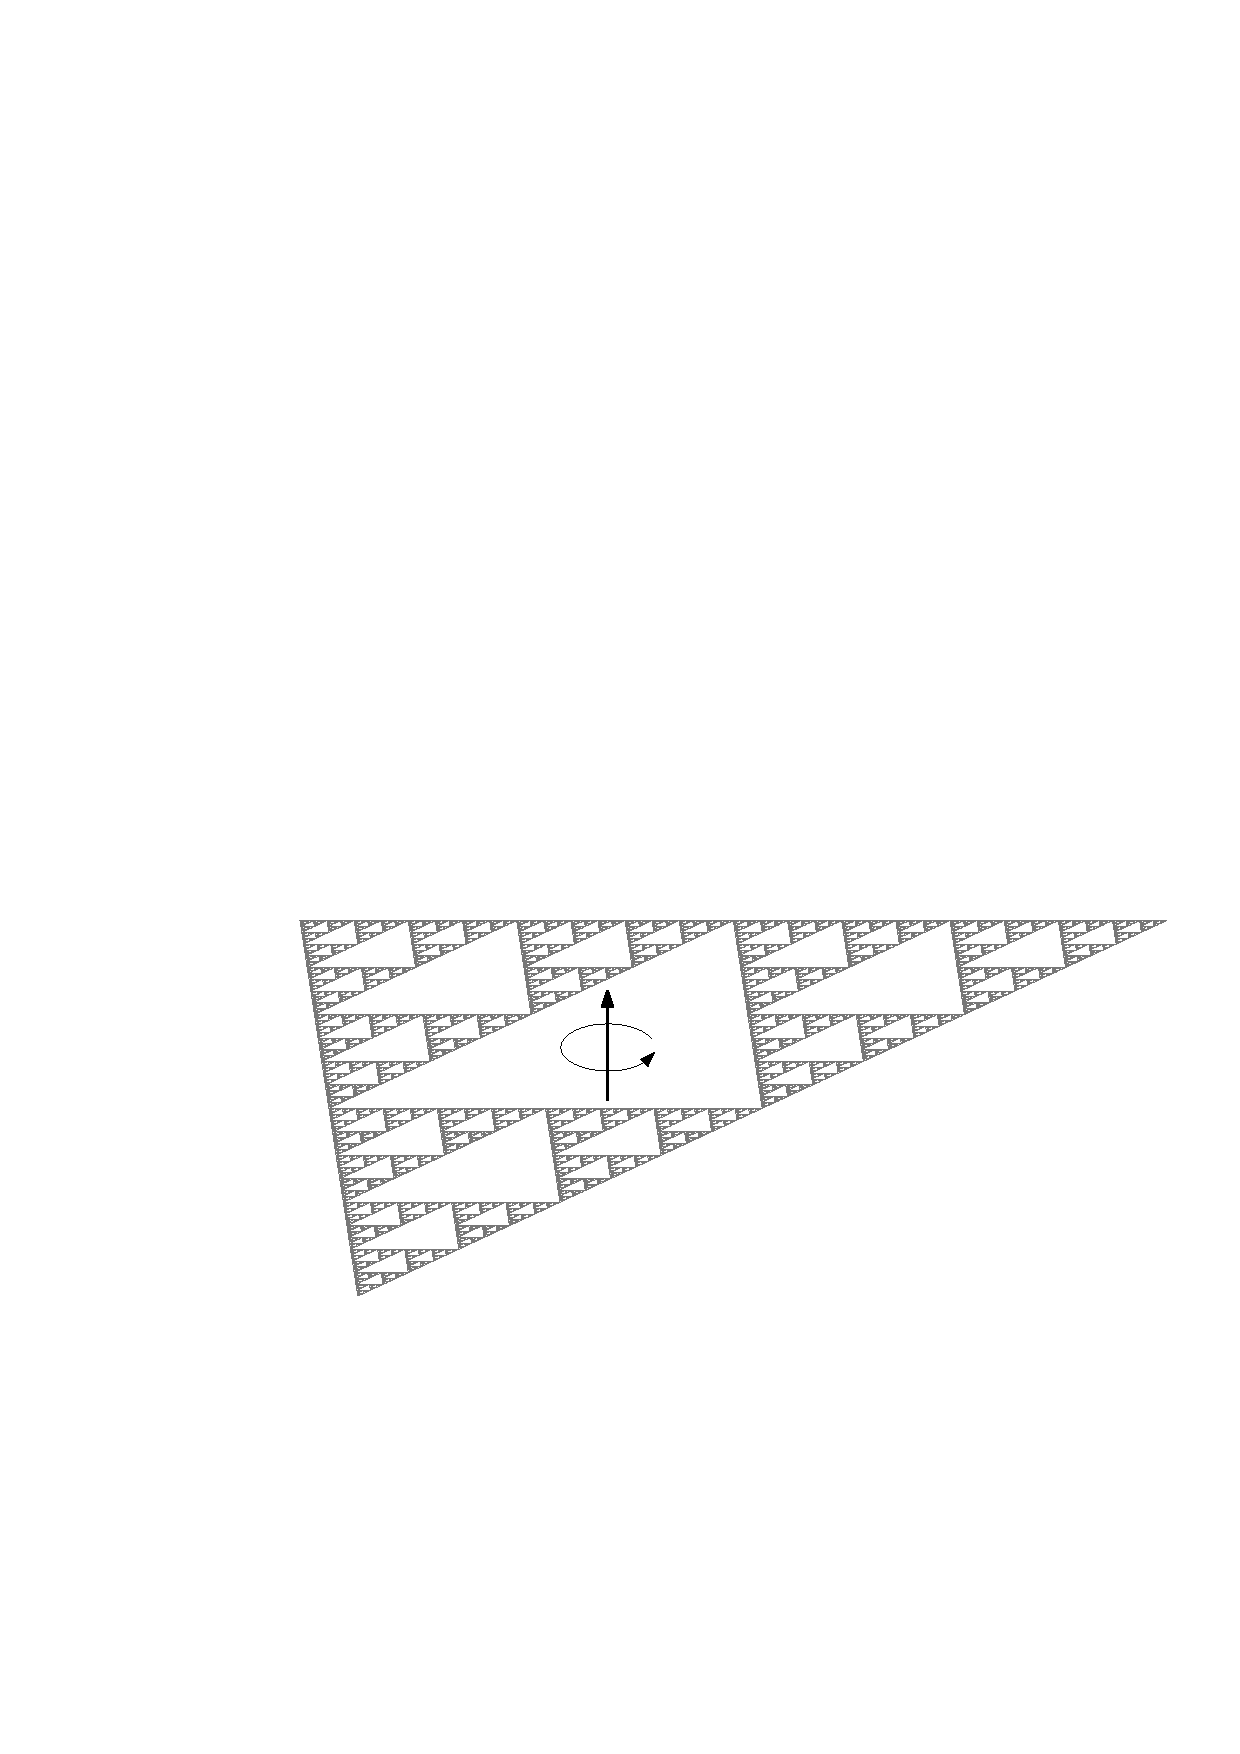
\includegraphics[width=7.5cm, height=3.5cm]{sd} 
\vspace*{3mm}\caption*{\rom{6}: Sierpinski triangle and rotational axis}
\end{subfigure}%
\begin{subfigure}{.5\textwidth}
\centering
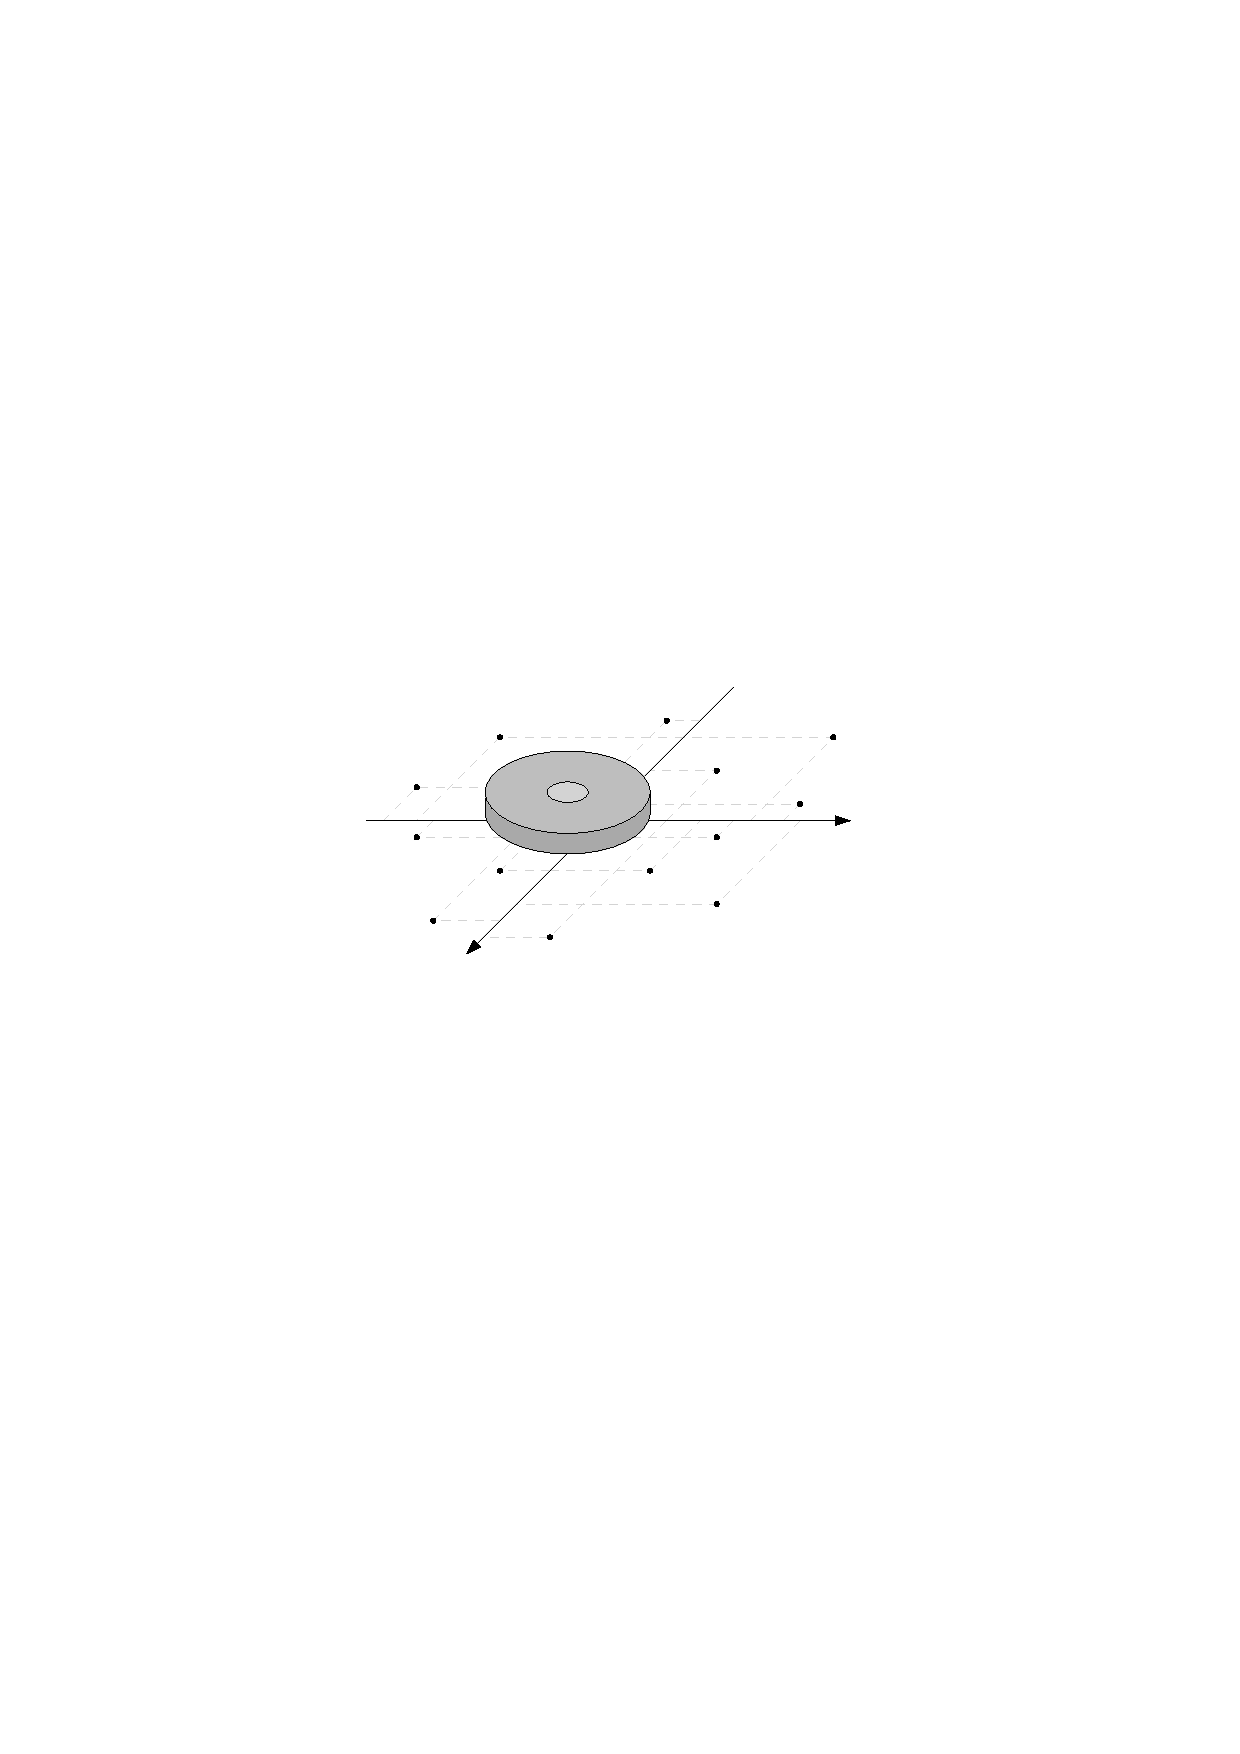
\includegraphics[width=7.5cm, height=3.5cm]{cl}
\vspace*{3mm}\caption*{\rom{5}: Curling stone on the infinite plane}
\end{subfigure}\vspace*{-0.5cm}
%\caption{Two subfigures}
\end{figure}


%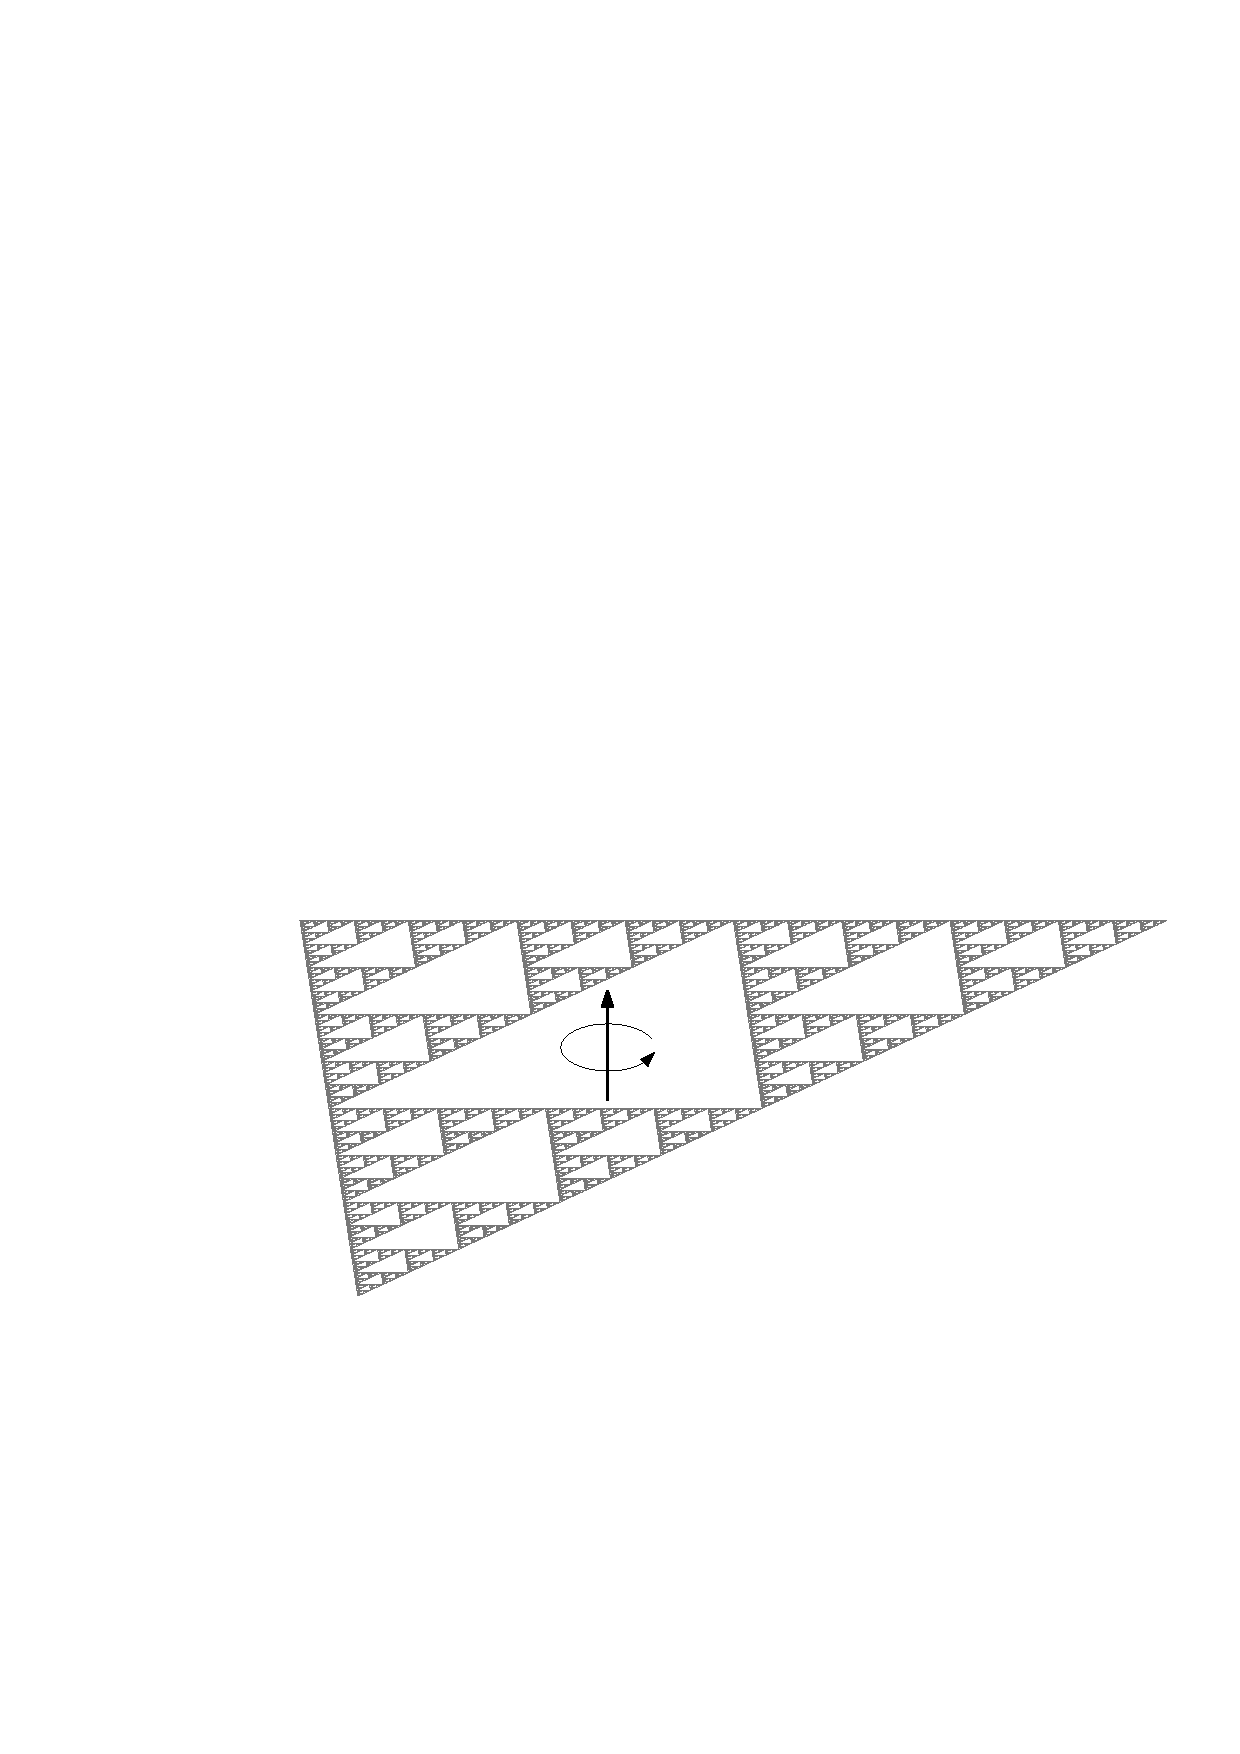
\includegraphics[width=5cm, height=5cm]{sd}
\end{document}


